\chapter{Debugging}

\begin{quote}
  \textit{Debugging is twice as hard as writing the code in the first place. Therefore, if you write the code as cleverly as possible, you are, by definition, not smart enough to debug it.}\begin{flushright}
    \tiny{Brian W. Kernighan}
  \end{flushright}
\end{quote}

Often times, it happens that a written program has different behaviour than we expected. This can manifest in all sorts of ways, from different output to crashing. There are many ways of finding the mistake, one of them is using a debugger to debug the program \cite{software-debugging-testing-verification}.
Debuggers can attach to existing process or spawn a new one. They often have functionalities like displaying variable/register values, allowing to read and write into program memory, change the executed code itself and to stop at some point in the program. Implementation of debuggers can vary based on target machine, operating system or if the program is native or expected to be run by an interpreter.

There are multiple debugger types \todo{Ocitovat tu microsoft press store thingie popr. kokesovo prednasky}.
\begin{itemize}
    \item An user-mode debugger - Can debug applications in user mode.
    \item A kernel debugger - Can debug the kernel and the kernel drivers.
    \item A source-level debugger - Can set breakpoints in application according to its source code.
    \item An assembly-level debugger - Works with the assembly language
\end{itemize}

This thesis will mainly focus on source-level debugging and assembly level debugging. We will see that those two are closely intertwined. First, we will present the most important and common debugger features.

\section{Fundamental debugger features}
\subsection{Breakpoint}\label{breakpoint}
Breakpoints are one of the most important debugger features. Source-level debugger can set them on some location in the source code and when the program arrives at that location, it will pause. The debugger can then inspect various traits of the running program. The location is most often line, but can even be inside expressions\footnote{This is especially important for functional languages, where function can just be one big expression.}. Hovewer we will consider breakpoints that only stops on a line. Assembly-level debuggers can stop when instruction on some address is being executed, so effectively on a line of the assembly program.

Breakpoints may also have conditions that are checked when the program arrives at a given line. If the condition holds then the program is paused. This can be useful for example to stop at the end of the loop.

\subsection{Stepping}
Debuggers also allow us to "make a step" in the code. It executes one line and pauses on the next one. This means that we can run the program line by line and inspect the behavior of the program.
There are often multiple categories of steps:

\begin{itemize}
    \item Step in - Executes one line. If the line was a call to a function, it pauses on the first line of the called function.
    \item Step over - Executes one line. If the line was a call to a function, it executes the whole body of the function and pauses on the line after the call instruction.
    \item Step out - Runs the program until it returns from current function, and pauses on that line.
\end{itemize}

\subsection{Inspecting and changing memory}
\todo{TODO}

\section{Debugging native programs}
For now, we pretended that source-level debuggers can magically work with lines of source code. However, for programs to be run they first need to be compiled to native code - a series of binary instructions (there are also interpreted programs, which we will touch upon later). The debugger then interacts with this native code. It, by itself, has no idea that line $x$ corresponds to address $y$. The compiler must embed this information in the executable, or somewhere else, for the debugger to know this type of information. One of such standards of encoding debug information is DWARF format \cite{dwarf}, which will be thoroughly described in \todo{TODO} section. 

As we mentioned, some debuggers only work on the assembly level. They do not perform any mapping to the source code. And the debuggers that do have to work with machine code all the same. In the next section, we will explore how assembly-level debuggers are implemented. The implementation itself can greatly differ based on the operating system or target machine. The following section aims to describe the most often used OS and targets.

\subsection{Breakpoints}
Term \textit{debuggee} means a program that is being debugged. The instuction architecture \textit{x86} contains special instruction \mintinline{c}{INT3}, opcode \mintinline{c}{0xCC}. When processor executes this instruction it issues special interrupt and advances program counter by one. The interrupt is then handled by OS. How the handling is done depends heavily on OS and will be covered later. 

Consider the following code \todo{Typeset these guys correctly}
\begin{minted}{asm}
0x0 xor    eax,eax        33 c0
0x2 mov    esp,ebp        8b e5
0x4 pop    ebp            5d
\end{minted}
To create a breakpoint on address \mintinline{c}{0x02}, the debugger needs to replace the code on that location with the \mintinline{c}{0xCC}. The result would look like this:
\begin{minted}{asm}
0x0 xor    eax,eax        33 c0
0x2 int3                  cc e5
0x4 pop    ebp            5d
\end{minted}
The processor executes the \mintinline{c}{xor}, then the \mintinline{c}{int3}, this sends the interrupt, but because that instruction was executed the program counter is now set to \mintinline{c}{0x3}. If the debugger would just told the program to continue it would execute the instruction at that point, which begins with \mintinline{c}{0xe5}. If the replaced instruction is one byte in size, it would skip the replaced instruction and execute the rest of the program. If it was bigger, it would essentially interpret the body of that instruction as new instruction. This would most likely cause a crash. The debugger needs to deal with this. 

\subsection{Trap flags}
The x86 architecture contains special \textit{Trap flag}. When it is set, the processor issues interrupt \mintinline{c}{INT1} every time an instruction is executed. \todo{Doplnit nebo smazat: Viz konzultace}.

\subsection{ptrace}
Linux offers special system call which is very handy for debugging. It is called \mintinline{c}{ptrace} \cite{ptrace} - process trace. It has following signature: \mintinline{c}{ptrace(PTRACE_COMMAND, pid, ...)}. It takes a \mintinline{c}{PTRACE_COMMAND}, which specifies the behaviour of the function (for example \mintinline{c}{PTRACE_SINGLESTEP} for single step), pid of some process and some other parameters, depending on the \mintinline{c}{PTRACE_COMMAND}. 

It allows to observe and control the execution of another process, which will most often be the debuggee. When the debugee is traced, it will stop each time a signal is delivered\footnote{\mintinline{c}{SIGKILL} is an exception, it will have its usual effect.}. The debugger will be notified at its next call to \mintinline{c}{waitpid}. This system call return value will indicate the reason debuggee stopped. \mintinline{c}{ptrace(PTRACE_TRACEME, ...)} called from a child of the debugger will cause the debugger to \textit{attach} to the child, which is the debuggee. The debugger can then issue other commands to the child. There are also \mintinline{c}{PTRACE_ATTACH} and \mintinline{c}{PTRACE_SEIZE}, which can be used for attaching to existing process.

\mintinline{c}{ptrace} has many commands, here are some of the most important:
\begin{itemize}
    \item \mintinline{c}{PTRACE_PEEKTEXT, PTRACE_PEEKDATA} - Read tracee's memory,
    \item \mintinline{c}{PTRACE_POKETEXT, PTRACE_POKEDATA} - Write into tracee's memory,
    \item \mintinline{c}{PTRACE_GETREGS} - Read tracee's register values,
    \item \mintinline{c}{PTRACE_SETREGSET} - Modify tracee's register values,
    \item \mintinline{c}{PTRACE_GETSIGINFO} - Retrieve information about the signal that caused tracee to stop,
    \item \mintinline{c}{PTRACE_CONT} - Restart the stopped tracee process,
    \item \mintinline{c}{PTRACE_SINGLESTEP} - Restart the stopped tracee but stop it after executing one instruction.
\end{itemize}

\todo{Describe how they are used in real code}

\subsection{Windows}
Windows also has built-in support for debugging at the Win32API layer \cite{windows-msdn-debugging-api, windows-press-debugging-api}.
It builds on \textit{debug events} and \textit{debug functions}. Summary of some of the functions that Win32 API offers which all help with debugging:

\begin{itemize}
    \item \mintinline{c}{DebugActiveProcess} - Attaches the debugger to an active process.
    \item \mintinline{c}{DebugBreakProcess} - Causes a breakpoint exception to occur in the specified process. 
                                          This passes control of the process to the debugger if there is one.
    \item \mintinline{c}{WaitForDebugEvent} - Waits for new debug events.
    \item \mintinline{c}{ContinueDebugEvent} - Continue the process execution after processing debug event.
    \item \mintinline{c}{OutputDebugString} - Sends a string to the debugger for display.
    \item \mintinline{c}{ReadProcessMemory} and \mintinline{c}{WriteProcessMemory} - Read and modify process virtual address space.
    \item \mintinline{c}{FlushInstructionCache} - Flushes instruction cache of the process.
\end{itemize}

The general structure of Windows debugger can be seen in figure \ref{fig:win32debugger}.
The debugger waits for debug events via function \mintinline{c}{WaitForDebugEvent}.
This function has a timeout parameter, so the debugger can also do other things while it's waiting.
These events are put in a queue, so the debugger will not miss any.

\begin{figure}
    \centering
    \scalebox{0.8}{
    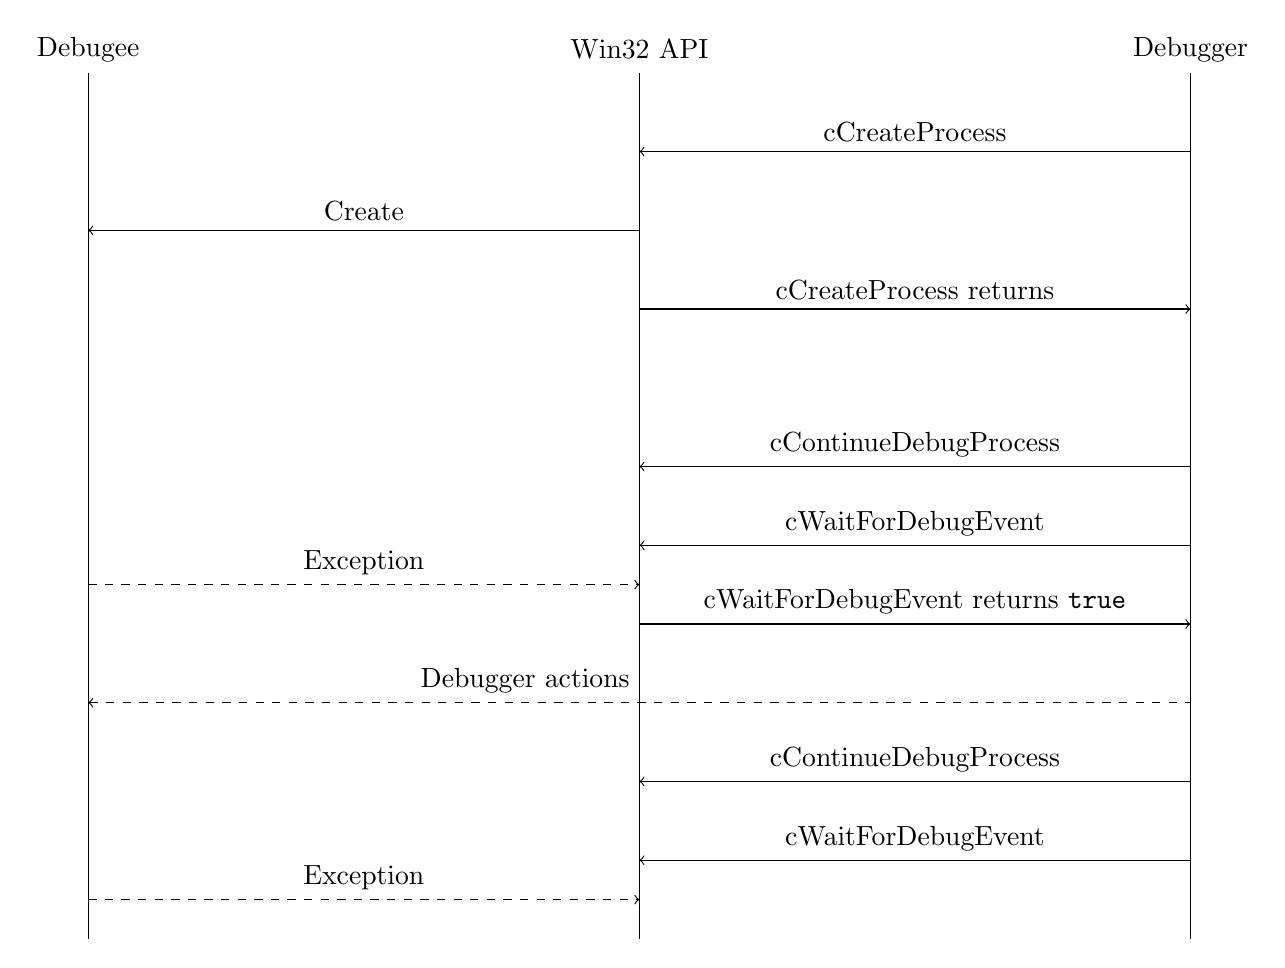
\begin{tikzpicture}
        \draw (-7,0) -- (-7,-11) (0,0) -- (0,-11) (7,0) -- (7,-11);
        \node at (-7,.3) {Debugee};
        \node at (0,.3) {Win32 API};
        \node at (7,.3) {Debugger};
        \draw[<-] (0,-1) -- node[midway,above] {\mintinline{c}{CreateProcess}} (7,-1);
        \draw[<-] (-7,-2) -- node[midway,above] {Create} (0,-2);
        \draw[->] (0,-3) -- node[midway,above] {\mintinline{c}{CreateProcess} returns} (7,-3);
        \draw[<-] (0,-5) -- node[midway,above] {\mintinline{c}{ContinueDebugProcess}} (7,-5);
        \draw[<-] (0,-6) -- node[midway,above] {\mintinline{c}{WaitForDebugEvent}} (7,-6);
        \draw[dashed,->] (-7,-6.5) -- node[midway,above] {Exception} (0,-6.5);
        \draw[->] (0,-7) -- node[midway,above] {\mintinline{c}{WaitForDebugEvent} returns \texttt{true}} (7,-7);
        \draw[dashed, <-] (-7, -8) -- node[above left] {Debugger actions} (7, -8);
        \draw[<-] (0,-9) -- node[midway,above] {\mintinline{c}{ContinueDebugProcess}} (7,-9);
        \draw[<-] (0,-10) -- node[midway,above] {\mintinline{c}{WaitForDebugEvent}} (7,-10);
        \draw[dashed,->] (-7,-10.5) -- node[midway,above] {Exception} (0,-10.5);
    \end{tikzpicture}
    }
    \caption{A sequence diagram for debugger using Windows api. Inspired by \todo{NI-REV 6. lecture}}
    \label{fig:win32debugger}
\end{figure}

The debug events are thoroughly described in subsection \ref{section:Debug Events}. The main point of interest is the exceptions.
By these, we do not mean the standard C++ exceptions but rather Microsoft \textit{Structured Exception Handling}.

\subsubsection*{Debug Events}\label{section:Debug Events}
Debugging events are various incidents in the debuggee that causes the system to notify the debugger \cite{windows-msdn-debug-events}. These are stored in special \mintinline{c}{DEBUG_EVENT} structure, which is received in \texttt{WaitForDebugEvent} call from debugger. This structure contains various information about the event, the internals can be seen on figure \ref{fig:DebugEvent}. These events include loading and unloading a DLL, creating and exiting a process, sending debug strings via the \mintinline{c}{OutputDebugString} and so on. It also includes exceptions, those are probably the most important for us. 
\begin{figure}
\begin{minted}{c}
typedef struct _DEBUG_EVENT {
  DWORD dwDebugEventCode;
  DWORD dwProcessId;
  DWORD dwThreadId;
  union {
    EXCEPTION_DEBUG_INFO      Exception;
    CREATE_THREAD_DEBUG_INFO  CreateThread;
    CREATE_PROCESS_DEBUG_INFO CreateProcessInfo;
    EXIT_THREAD_DEBUG_INFO    ExitThread;
    EXIT_PROCESS_DEBUG_INFO   ExitProcess;
    LOAD_DLL_DEBUG_INFO       LoadDll;
    UNLOAD_DLL_DEBUG_INFO     UnloadDll;
    OUTPUT_DEBUG_STRING_INFO  DebugString;
    RIP_INFO                  RipInfo;
  } u;
} DEBUG_EVENT, *LPDEBUG_EVENT;
\end{minted}
\caption{Structure which contains info about debug event.}
\label{fig:DebugEvent}
\end{figure}

\subsubsection*{Structured Exception Handling}
This feature is specific to Windows only. For example, if division by zero was performed in a program on Linux,
a signal would be sent to the process. Windows don't have signals, instead, it uses Structured Exception Handling \cite{windows-msdn-seh}. 
From now on, we will be using the abbreviation 'SEH'.
An exception is an event that requires execution of code outside the normal flow of control. There are software exceptions,
like throwing an exception explicitly or by OS, and hardware exceptions, like the division by zero we mentioned.
Instruction with opcode \mintinline{c}{0xCC}, which is used for breakpoints, will also raise an exception. SEH unifies both of these things into one.

When an exception is triggered, control is transferred to the system. It saves the state of the thread and some other information.
This information can be used to continue execution from the point where the exception was thrown when it is resolved. It also
contains information about which type of exception was thrown, if execution can continue after handling the exception, address where the
exception occured and some others\footnote{See MSDN documentation \cite{windows-msdn-seh} for full detailed list}.
The system then searches for an exception handler which will handle the exception. The search is performed in this order:

\begin{enumerate}
    \item If the process is debugged the debugger is notified.
    \item If it is not or the debugger does not handle the exception, the frame-based exception handler is to be found\footnote{The handlers are not very important to us, see MSDN documentation if you're interested \cite{windows-msdn-seh}.}
    \item If no frame-based handler can be found, or no handler handles the exception, but the process is being debugged then the debugger gets notified once again.
    \item The system provides default handling, which is to terminate the program via \mintinline{c}{ExitProcess} most of the time.
\end{enumerate}

Here we see that every exception that occurs in the debuggee causes the debugger to be notified. Breakpoints are also caused by an exception, as was briefly mentioned before. There are two possible notifications to the debugger. The first is known as \textit{first-chance} notification \cite{windows-msdn-dbg-exc-handling}. The debugger can (and should) inspect the information about the exception and see if it was a breakpoint or single-step. These only occurs if the process is debugged (it wouldn't happen otherwise) and the debugger should handle them. If it is something else it can ignore the exceptions. When the program is continued via \mintinline{c}{ContinueDebugEvent}\footnote{This function has a special parameter, which is used to tell that the exception was or was not handled.}, the debugger is notified once again if no appropriate exception handler was found for the exception. This is known as \textit{last-chance} notification because if the debugger does not handle the exception the debuggee will be terminated. It gives the user a chance to debug why is his process terminating.

Here are some exceptions that tie into debugging:
\begin{itemize}
    \item \mintinline{c}{STATUS_BREAKPOINT} - Raised when a hardware-defined breakpoint was encountered. This includes the mentioned \mintinline{c}{INT3} instruction.
    \item \mintinline{c}{STATUS_SINGLE_STEP} - Raised when a single step was completed, ie. when instruction was executed and the trap flag is set.
\end{itemize}

\subsubsection*{Tying it all together}
Now we have all necessary building block to build a simple proof of concept Windows debugger. On figure \ref{fig:windows-debugger-mainloop}, you can see a basic idea of a main loop of the debugger. It waits for debug events and branches depending of the type of event. It needs not only handle exceptions, but other events also. For example if the debugee creates a thread that is something the debugger should be aware of. Modern debuggers trace all threads of the program.

\todo{Pridat dalsi figure kde je jak se hanndlujou tyhle blbosti} However, exceptions are the most interesting for us. There, breakpoint and single step handling should be done. On both of these, the debugger should handle the exception itself, so this is the \textit{first chance} notifications. There is also an \mintinline{DBG_CONTROL_C}, which happens on CTRL + C keyboard press. This should terminate the program. The debugger will pass the first chance and catch the last chance exception, so user has a final chance to look at the program state before it exits.

\begin{figure}
    \begin{minted}{c}
void EnterDebugLoop(const LPDEBUG_EVENT DebugEv)
{
   DWORD dwContinueStatus = DBG_CONTINUE; // exception continuation 
   for(;;) 
   { 
      WaitForDebugEvent(DebugEv, INFINITE); 
      switch (DebugEv->dwDebugEventCode) 
      { 
         case EXCEPTION_DEBUG_EVENT: 
            // Handle exception debug events
         // Other debug events
      } 
   ContinueDebugEvent(DebugEv->dwProcessId, 
                      DebugEv->dwThreadId, 
                      dwContinueStatus);
   }
}
\end{minted}
\caption{Windows debugger main loop}
\label{fig:windows-debugger-mainloop}
\end{figure}

